\begin{previewactivity}[\textbf{Venn Diagrams for Two Sets}]\label{PA:venn} \hfill \\
In \typeu Activity~\ref*{PA:setops}, we worked with verbal and symbolic definitions of set operations.  However, it is also helpful to have a visual representation of sets.  \textbf{Venn diagrams} are used to 
\index{Venn diagram}%
  represent sets by circles (or some other closed geometric shape) drawn inside a rectangle.  The points inside the rectangle represent the universal set  $U$, and the elements of a set are represented by the points inside the circle that represents the set.  For example, Figure~\ref{fig:venn2-prev} is a Venn diagram showing two sets.
\begin{figure}[h]
\begin{center}
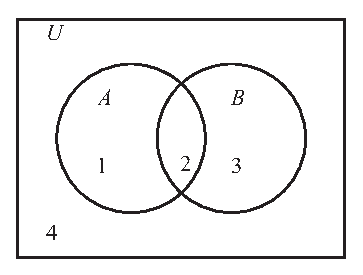
\includegraphics{figps-venn2.eps}
\caption{Venn Diagram for Two Sets} \label{fig:venn2-prev}
\end{center}
\end{figure}

\noindent
In Figure~\ref{fig:venn2-prev}, the elements of  $A$  are represented by the points inside  the left circle, and the elements of  $B$  are represented by the points inside  the right circle.  The four distinct regions in the diagram are numbered for reference purposes only.  (The numbers do not represent elements in a set.)  The following table describes the four regions in the diagram.
$$
\BeginTable
\BeginFormat
| c | l | c |
\EndFormat
" Region  "  Elements of $U$  "   Set  " \\ \_
"1  "  In $A$ and not in $B$  "  $A - B$  " \\
"2  "  In $A$ and in $B$	"  $A \cap B$  " \\
"3  "  In  $B$  and not in $A$  "  $B - A$  " \\
"4  "  Not in $A$ and not in $B$ "	$A^c  \cap B^c $ " \\
\EndTable
$$
We can use these regions to represent other sets.  For example, the set  $A \cup B$  is represented by regions 1, 2, and 3 or the shaded region in Figure~\ref{fig:union2}.
\begin{figure}[h]
\begin{center}
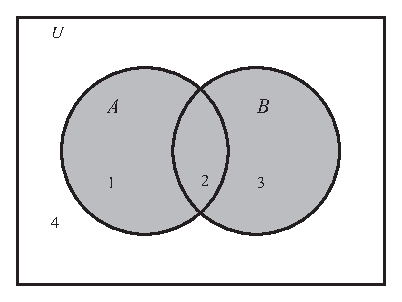
\includegraphics{figps-aunionb.eps}
\caption{Venn Diagram for $A \cup B$} \label{fig:union2}
\end{center}
\end{figure}

\newpage
\noindent
Let $A$ and $B$ be subsets of a universal set $U$.  For each of the following, draw a Venn diagram for two sets and shade the region that represent the specified set.  In addition, describe the set using set builder notation.
\begin{multicols}{3}
\begin{enumerate}
%\item $A \cap B$
\item $A^c$
\item $B^c$
\item $A^c \cup B$
\item $A^c \cup B^c$
\item $\left( A \cap B \right)^c$
\item $\left( A \cup B \right) - \left( A \cap B \right)$
\end{enumerate}
\end{multicols}
\end{previewactivity}
\hbreak
\endinput

